\chapter{Распределение интеллектуальных ресурсов со схемой параллельного обучения для гетерогенных сетей стандарта LTE Smallcell} \label{chapt2}

\section{Одиночное изображение} \label{sect2_1}


\section{Общее описание} \label{sect2_1}
Эффективное управление радио ресурсами и схемами координации помех стало важным требованием для успешного внедрения гетерогенных сетей с малыми сотами. При таком подходе, развернуто большое количество маломощных устройств, с целью увеличения повторного использования пространственных частот из выделенной области. В данной статье мы предлагаем распределенную мультиагентную стратегию, где малые соты локально контролируют использование ресурсов для максимизации общей пропускной способности системы. Главная цель - обеспечить каждую соту умением принимать решение самостоятельно, учитывая занятость ресурсов окружающих сот. Мы изучаем сосуществование с некооперативной макросредой и предлагаем механизм повышения эффективности обучения с помощью процедуры интеллектуальной безопасной смены. Мы иллюстрируем применение этой стратегии обучения для выделения поддиапазонов и предлагаем несколько механизмов повышения скорости конвергенции при отсутствии связи. Результаты предложенного метода оцениваются в случае установок LTE и сравниваются с рядом традиционных схем распределения ресурсов. Моделирования на уровне системы показывают, что она обеспечивает значительное улучшение производительности системы для разнородного внедрения с невзаимодействующими агентами, не нанося ущерба для эффективности системы.


\section{IEEEkeywords}
LTE, интерференция между сотами (ICI), управление ресурсами, обучение с подкреплением, обмен ресурсов, соотношение сигнала и шума, пропускная способность, частотно-временной анализ, распределение ресурсов, плотные сети LTE

\section{Введение}
%\blindtext

Растущий спрос на поддержание высокого качества услуг беспроводных сотовых технологий создает реальную проблему для развивающихся LTE-А сетей~\cite{TS36.300}.
Концепция малых сот считается самым практичным способом увеличения общей пропускной способности системы. В этом подходе большое количество маломощных устройств (малые соты) используется для увеличения повторного использования пространственных частот и улучшения местного покрытия. Эта концепция принципиально меняет требования к работе системы сотовых сетей. Довольно часто малые соты развернуты без или с небольшим объемом управления от оператора сети. Это вызывает необходимость адаптировать интеллектуальное управление радио ресурсами для малых сот на должном уровне.
Одним из основных технических требований, предъявляемых к современным сотовым системам, является максимизация фактора повторного использования частот ~\cite{M.1645}. Скудный лицензированный спектр безусловно приводит к перекрытию диапазонов частот и интерференции между сотами (ICI). В сфере контроля интерференций и ликвидации их последствий осуществляется интенсивная научная деятельность. В промышленности эти усилия были в основном приняты в виде строгого статического разделения частот или реактивного (в отличие от активного) ручного управления доступным спектром.
Понятие малых сот является проблемным для многих традиционных представлений о структуре сетей сотовой связи ~\cite{6211486}. В дополнение к обширному уплотнению, устройства теперь могут часто включаться и выключаться, что вызывает частые неконтролируемые изменения в структуре сети. Таким образом, нельзя больше применять привычные подходы к контролю интерференций, поскольку они основаны на предположениях равномерного гексагонального внедрения и статически централизованного управления базовыми станциями. Вместе с ростом числа устройств увеличивается количество надземных сервисов. В таких условиях использование централизованных решений становится гораздо менее благоприятным, а распределенные алгоритмы для вмешательства и управления ресурсами являются более перспективными.
В этой статье мы предлагаем подход к активизации вышеупомянутых динамических схем распределения ресурсов с распространенной двухуровневой процедурой обучения. Мы направлены на использование только местной информации и ограничение обмена информацией с соседними сотами. По замыслу, каждой соте соответствует уникальный набор правил распределения ресурсов, что позволяет всей системе сойтись быстрее. Каждый учебный посредник исследует окружающую среду, различая ответы от соперничающих посредников и невзаимодействующих базовых макро станций. Эти дополнительные знания затем используются, чтобы выбрать наиболее подходящее распределение поддиапазона.
Основной вклад данной работы заключается в следующем. Предложен новый метод для координации помех в плотных гетерогенных сетях. Должным образом рассмотрены две типичные проблемы в большинстве параллельных схем обучения - разрастание учебного пространства и блокирование возможности обследования. Предложенный алгоритм осуществляет мониторинг местного уровня интерференции, использование ресурсов и выделяет блоки физических ресурсов оптимальным образом. Алгоритм является полностью распределенным и, в частности, предполагается отсутствие связи между сотами. Алгоритм быстро адаптируется к изменению интерференции и внешних условий сети, что делает его очень практичным. Сходимость и быстродействие алгоритма вычисляются путем моделирования.
Эта статья организована следующим образом. В разделе II представлена соответствующая работа. Раздел III описывает предложенный алгоритм и обеспечивает некоторую интуицию по теме ключевых проектных решений. В разделе IV приводятся параметры среды моделирования и оценки результатов. Наконец, мы заключаем с общими замечаниями в разделе V.

\section{Соответствующая работа}
В данном разделе представлена соответствующая работа в области управления радио ресурсами и интерференции внутри малых сотовых сетей. Существует множество исследований по данной теме, в особенности, на интерференции меду сотами, которая является одним из самых сдерживающих факторов в ситуациях, касающихся плотных малых сот. Нами были найдены многочисленные исследовательские работы о деятельности в этой области, посвященные управлению вмешательства в гетерогенных сетях. Полный обзор основных методов управления ICI, совместимых с LTE, может быть найден в ~\cite{cite_overview}.

Для плотных несогласованных внедрений управление интерференцией между сотами является более сложным, чем в обычных макро-сотовых сетях. Одним из перспективных методов управления радио ресурсами является действия систем сот, с целью узнать их беспроводное окружение. Затем извлеченные данные могут быть использованы для непосредственного принятия решений (как в \cite{mab}) или (как, например, в \cite{q-learning}) для получения схемы ответа о состоянии работы, чтобы самостоятельно достичь оптимального распределения ресурсов. В частности, в работе \cite{q-learning} сообщается о самоорганизации и управлении распределенных интерференций для фемтосот, которые делят имеющиеся радиосредства с макроэлементами. Рассмотрен многоагентный подход к обучению на основе распределенного Q - обучения. Малые соты меняют свою мощность передачи, чтобы максимизировать суммарную мощность, в то время как агрегированные помехи нисходящей линии связи, образованные на ресиверах макро пользователей поддерживаются в заданных пределах.

В \cite{mp-qlearning} и \cite{fzq-learning} авторы предлагают другие схемы на основе Q-обучения и демонстрируют значительную выигрышность по сравнению с обычными методами повторного использования частот с точки зрения пропускной способности для пользователей сотовых сетей. Однако, эти методы устанавливают жесткие требования по качеству обратной связи с пользователями и становятся менее эффективными с точки зрения времени сходимости в динамичных случаях с гибким трафиком. 

В \cite{mab} предложен подкрепленный подход к обучению, где базовые станции автономно выбирают наиболее спектрально уместные ресурсы. Это позволяет гибко управлять компромиссом между изучением окружающей среды и использованием накопленных знаний о нем. Подобные схемы с возможностью собственной конфигурации и самооптимизации также были предварительно представлены в \cite{local-area}, где алгоритм позволяет сотам динамически выбирать начальные куски спектра и опирается на механизмы контроля мощности. Управление интерференцией между сотами было также изучено в \cite{on-uplink}, где авторы предложили схему планирования с фиксированными вероятностями распределения. В данном случае, сложность предлагаемых стохастически схем управления радио ресурсами является относительно низкой, поскольку они предлагают децентрализованный подход и требуют только ограниченный объем передачи сигналов вещания. Однако, эти схемы могут быть неэффективными при рассмотрении большого размера сети малых сот.
Еще один интересный децентрализованный подход был предложен в ~\cite{1666484}, где проблема распределения каналов является эквивалентной для раскраски графа. Единственная информация, необходимая алгоритму, - обратная связь по уровню интерференции на выбранном канале. В~\cite{Duffy:2008:CAD:1377038.1377164} и ~\cite{4177619}сложность и скорость сходимости изучены на классе децентрализованных алгоритмов раскраски. Отметим, что проблема, рассматриваемая в данной статье, не может быть сведена к раскраске графа, так как соты могут находиться на одном и том же поддиапазоне, а в поддиапазонах границы частот не фиксируются.
В то время как некоторые решения обеспечили подходы к управлению распределением ресурсов, эти решения не дотягивают по отношению к ряду проблем, рассматриваемых в нашей работе. Предлагаемый способ предположительно преодолеет несколько ощутимых недостатков мультиагентного обучения. Основной проблемой является несоответствие между общей системой состояния и поведением агента. В перспективе сближения система имеет два состояния - разведочное, где изучение движет системы к стабильному состоянию, и состояние эксплуатации - стабильное состояние, где эффективность обучения низка в связи с необходимостью сохранить стабильность системы. Недостатком такого подхода является то, что система интенсивно изучает среды в одном состоянии (где распределение определяется, главным образом, исследованием поведения окружающих агентов), а затем работает в различных состояниях (определяется эксплуатационным поведением агентов). В этой статье мы предлагаем первоначально заставить группу агентов вести себя уникальным образом, чтобы добавить больше смысла в процесс обучения. Мы также изучаем еще одну проблему схемы обучения, которая заключается в разрастании и перерождении образовательного пространства с увеличением на ряд поддиапазонов.
Цель этого исследования заключается в получении согласованной схемы взаимодействия с акцентом на сосуществовании для плотной малой сотовой сети посредством распределения ресурсов путем введения нескольких новых усовершенствований в поведение обучения агентов.

\section{Интеллектуальное распределение ресурсов: \\алгоритм безопасной смены}
\subsection{Архитектура системы}
В этой статье мы рассмотрим технологии LTE/LTE-А сетей с разнородным внедрением базовых станций, таких как макросоты и малые соты, как показано на Рис.~\ref{fig:architecture}. Последняя обычно используется для улучшения покрытия макросот в помещениях и для повышения мощности в густонаселенных районах. Основной упор в данной работе сделан на сосуществование малых сот с макросредой, а также с невзаимодействующими малыми сотами различных поставщиков.

\begin{figure}[]
    \centering
    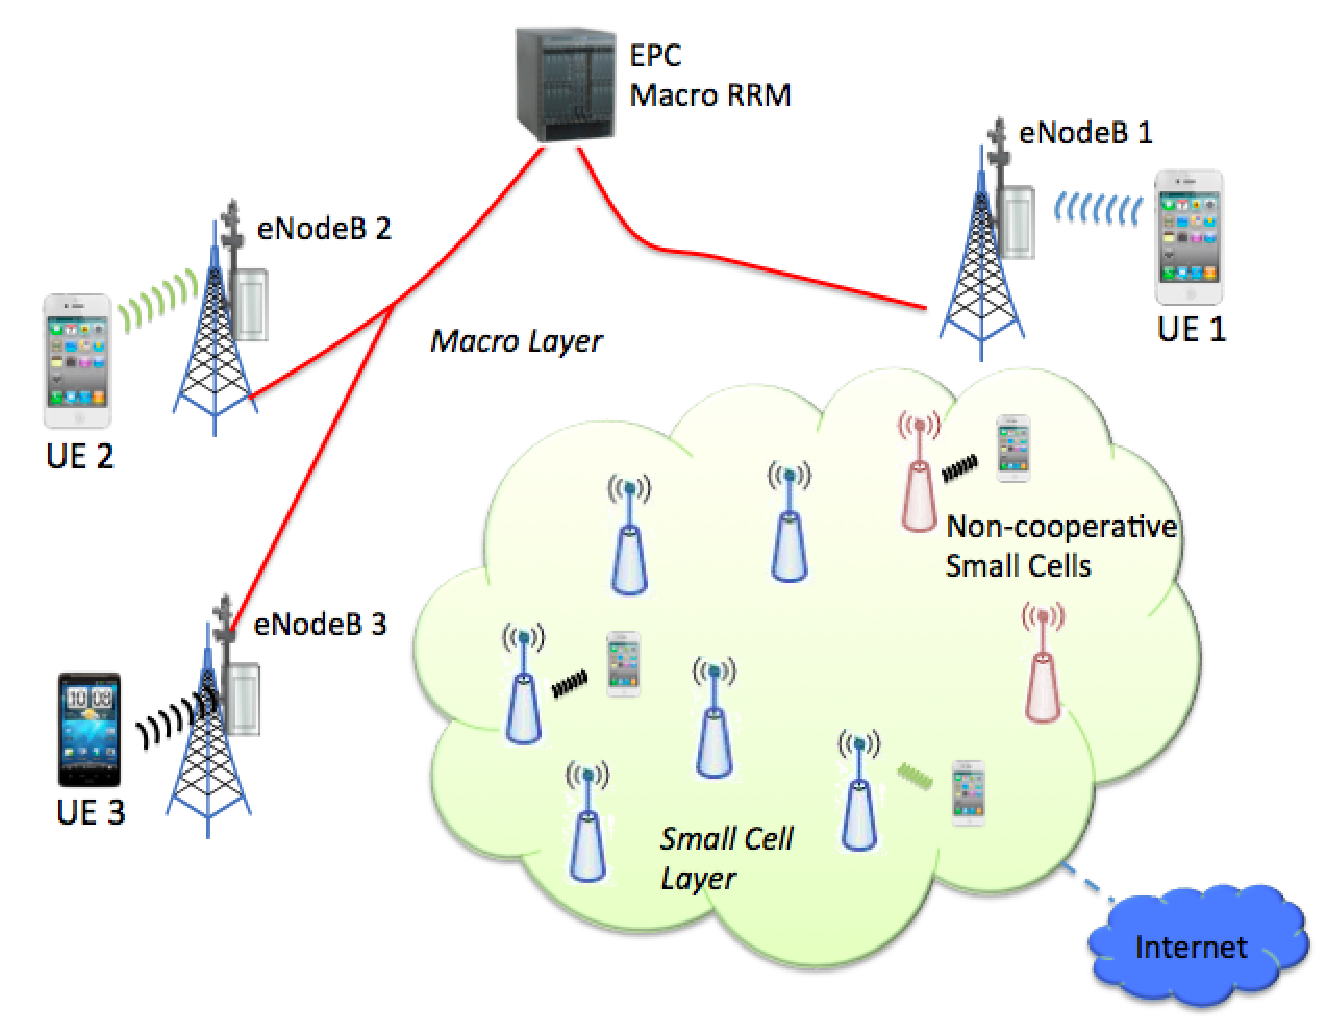
\includegraphics[width=8cm]{gcimages/architecture}
    \caption{Overall system setup: macro layer and small cell layers (cooperative and non-cooperative)}
    \label{fig:architecture}
\end{figure}

Рис.~\ref{fig:architecture} иллюстрирует типичный сценарий развертывания гетерогенных сетей~\cite{6824744}, которые обычно встречаются на практике. Они состоит из следующих элементов:

\begin{itemize}
\item[$\cdot$] Базовые макро станции (или eNodeB), которые используются для обеспечения основного покрытия сотовой сети. Базовые станции обычно оснащены готовым планом радио ресурсов, полученным на предварительном этапе радио-планирования. Объем услуг базовых станций обычно ограничивается на краях соты и в закрытых помещениях из-за потерь пути и многолучевого замирания. 
\item[$\cdot$] Малые соты (or HeNBs)- базовые станции малой дальности, которые в основном развернуты в комнатных условиях. Несогласованность монтажа и эксплуатации являются одним из наиболее привлекательных особенностей малых сот.
\item[$\cdot$] Невзаимодействующие соты - отдельный класс сетевых элементов, которые являются статически настроенными сотовым оператором или по какой-то причине действующие в рамках иных наборов правил, нежели малые соты. В данной работе эти агенты (наряду с другими источниками помех) дают ответ в макросреде.
\item[$\cdot$] Абонентское оборудование (UEs) - здесь мы не отмечаем различий между пользователями макросот и малых сот. Мы предполагаем, что пользователя всегда обслуживают базовые станции с сильным сигналом (что на практике в большинстве случаев является верным)
\item[$\cdot$] Транспортная инфраструктура: базовые макро станции подключаются к пакетному ядру оператора (ЕРС) через выделенную линию, тогда как малые соты соединены через интернет. Этот факт делает управление распределенными системами более практичным для малых сот.
\end{itemize}

\subsection{Системные требования}
В этой статье мы предъявляем следующие требования:
\begin{enumerate}
\item алгоритм должен адаптироваться к различным схемам внедрения, условиям макросреды и типам трафика~\cite{TS36.300}.
\item отсутствие вмешательства или подготовительной конфигурации не должны быть затребованы как самоорганизующиеся требования~\cite{TS36.902}.
\item отсутствие связи с посторонними агентами разрешено, чтобы избежать проблем транспортной сети, а также несовместимости с проприетарными интерфейсами.
\item скорость сходимости алгоритма должна быть сопоставима с типичной скоростью изменений в системе.
\end{enumerate}

\subsection{Управление системой}
\begin{figure}[h]
    \centering
    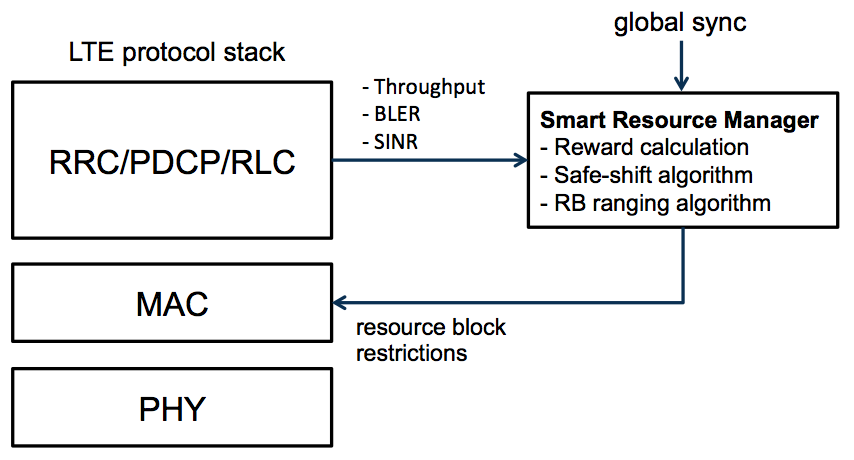
\includegraphics[width=8cm]{gcimages/algo_arch}
    \caption{Algorithm structure within LTE protocol stack: PHY - physical layer, MAC - media access layer, RRC/PDCP/RLC - higher levels providing performance feedback}
    \label{fig:algo_arch}
\end{figure}

На Рис.~\ref{fig:algo_arch} представлена упрощенная структура алгоритма в стеке протоколов сети LTE. Можно заметить, что не использованы входящие или исходящие каналы управления. Тем самым предлагаемое решение не предполагает каких-либо требований по качеству связи между базовыми станциями, так как оно предназначен для работы локально на каждой малой соте.
Общий принцип алгоритма заключается в следующем. Основываясь на статистику производительности от слоя L2~\cite{TS36.300} (например, BLER, спектральная эффективность) каждая малая сота самостоятельно принимает решение о блоке ресурсов для последующего периода времени. Единственный внешний входящий канал управления является глобальным источником времени. Он используется для выполнения синхронных операций (безопасной смены) в пределах группы малых сот. После принятия решения о распределении ресурсов в каждой соте, все разрешенные блоки ресурсов распределяются между пользователями на нижнем слое MАС-планировщиком.

\subsection{Схема распределения радиоресурсов}
В этой статье мы рассмотрим многоуровневые сети LTE составленные из множества малых сот, сосуществующих с окружающими базовыми макро станциями. Базовые макро станции и малые соты работают в одном частотном диапазоне, чтобы увеличить повторное использование пространственной частоты.

Для координации интерференции между соседними сотами каждая малая сота автономно принимает решения о распределении частот. Весь доступный частотный диапазон разбивается на ряд поддиапазонов. Эти поддиапазоны отмечены $b_{j}$, где $j=1, .., N$ и $N$ - общее количество поддиапазонов. Многопользовательское планирование ресурсов внутри каждой базовой станции осуществляется путем пропорционального справедливого планировщика.

В момент времени $t$ автономный агент должен решить, какой поддиапазон $b(t+1)$ из имеющегося спектра доступен для использования в следующем шаге $t+1$. Мы предлагаем схемы обучения распределению ресурсов, состоящие из двух уровней (см. Рис.~\ref{fig:algo_arch}):

\begin{itemize}
\item[$\cdot$] параллельное обучение с подкреплением~\cite{4445757}, с $N\times N$ матрицей перехода $T(t)$. Оно определяет вероятность перехода агента от поддиапазона $i$ к поддиапазону $j$ в момент времени $t$. Элементы матрицы периодически обновляются полученными наградами $RW_{ij}(t) = e^{(C_i(t-1) - C_j(t))}$, где $C_j(t)$ - достигаемая пропускная способность или количество пользователей с удовлетворенными требованиями QoS в момент времени $t$ при использовании поддиапазона $j$.
\item[$\cdot$] исследования макросред (см. разд.~\ref{sec:safe_shift}), более высокий уровень алгоритма с неинтерферирующим исследованием макросреды, где обучаемые агенты синхронно выполняют согласованные смены распределения (безопасные смены). $RW_{ij}(t_{sh})$ рассчитывается точно так же, как $RW_{ij}(t)$, но во время выполнения безопасной смены. Этот шаг отвечает за сосуществование с невзаимодействующими агентами и исследование макросреды.
\end{itemize}

Матрица перехода $T$ определяет вероятность перехода из поддиапазона $i$ к поддиапазону $j$. Значения $T_{ij}(t)$ и $T_{ij}(t_{sh})$ обновляются на каждой итерации (каждые 1 мс) на основе функции вознаграждения как в ~(\ref{eq:tm_update}).
\begin{equation}
    \label{eq:tm_update}
    T_{ij}(t) = (1-\alpha-\beta)T_{ij}(t-1) + \alpha RW_{ij}(t) + \beta RW_{ij}(t_{sh})
\end{equation}
\begin{equation}
    \label{eq:tm_update_c}
    RW_{ij}(t) = e^{(C_i(t-1) - C_j(t))}
\end{equation}
где:

\begin{itemize}
\item[$\cdot$]$ \alpha$ - коэффициент обучения, определяющий скорость сходимости алгоритма и коэффициент исследования и этапов эксплуатации. Оптимальное значение для этого параметра подбирается экспериментально в ходе симуляций.
\item[$\cdot$] $\beta$ - коэффициент обучения ($\beta < \alpha$) для макросред, определяющий сходимость алгоритма высшего уровня.
\end{itemize} 

В то время как соты не имеют одинаковых знаний об уровне занятости/интерференции каждого поддиапазона, матрица перехода $T$ обновляется независимо для каждой соты. В определенной степени, это может привести к уменьшению скорости сходимости алгоритма. Моделирования показывают, что этим поведением можно эффективно управлять с помощью тонкой настройки коэффициентов обучения. В следующем разделе предложен дополнительный метод для повышения скорости сходимости алгоритма.

\subsection{Ответ макросреды: случай безопасной смены}
\label{sec:safe_shift}
Любой агент обучения воспринимает ответ окружающей среды $\gamma = \gamma^{CL} + \gamma^{ML}$ состоящий из двух частей: $\gamma^{CL}$ - ответ, определяемый поведением соседних агентов, а $\gamma^{ML}$ - независимый ответ, определяемый слоем макросреды.
Рисунок \ref{fig:channel_exploration_blocked} иллюстрирует простой случай так называемой блокировки канала, где разведка окружающей среды заблокирована превосходством $\gamma^{CL}$, обусловленным выбором диапазона постороннего агента. Аналогичным образом на практике подавляющее большинство попыток разведки будут заблокированы ответом канала $\gamma_b^{CL}$ соседей. 

\begin{figure}[h!]
    \centering
    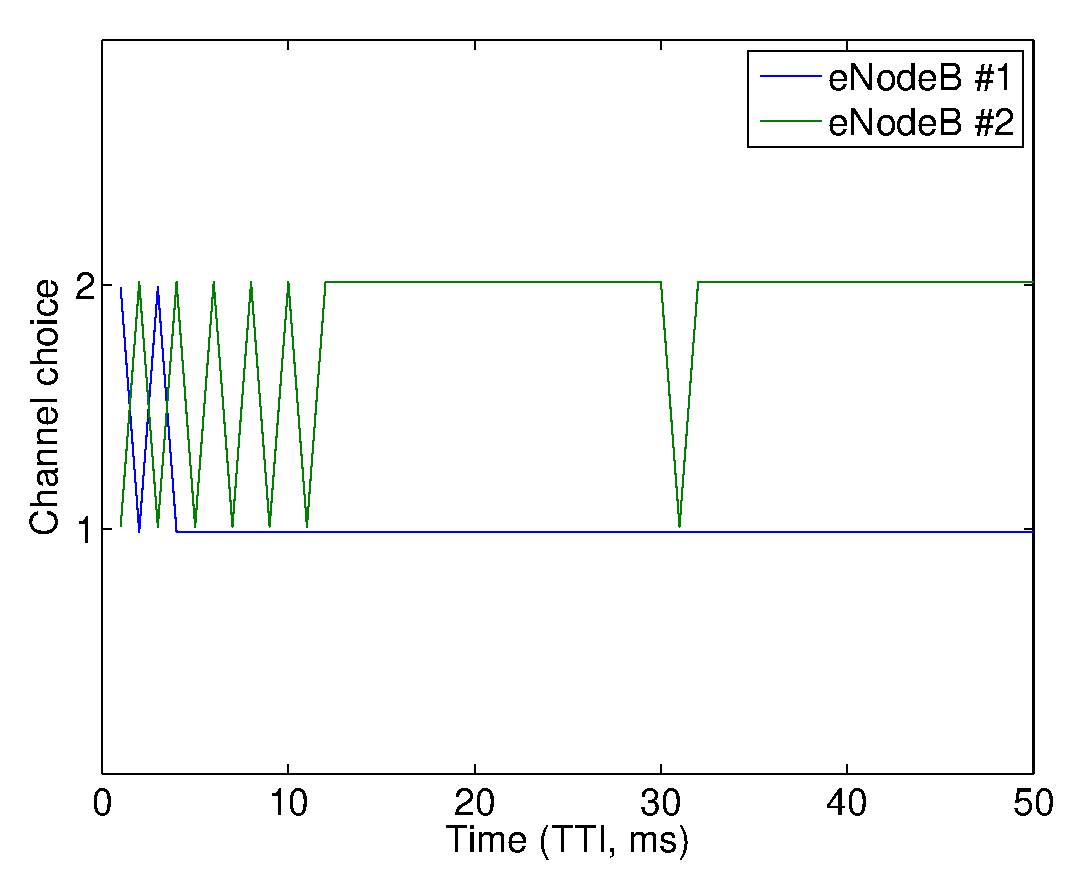
\includegraphics[width=8cm]{gcimages/channel_exploration_blocked}
    \caption{Example of channel exploration blocking. Both subbands are blocked.}
    \label{fig:channel_exploration_blocked}
\end{figure}

Чтобы справиться с описанным эффектом мы заставляем каждого агента изучать ответ макросреды $\gamma_b^{ML}$ в пределах каждого параллельного этапа обучения $t$ - процедура безопасной смены. При этом мы одновременно вынуждаем каждый агент последовательно изучить поддиапазоны ${(b_{t+1}+i)~mod~N}, i=1..N$. Очевидно, что это дополнение не влияет на $\gamma^{CL}$ компонент ответа, так как агенты на пересекающихся диапазонах в момент времени $t$ по-прежнему используют те же поддиапазоны в момент времени ${t+1}$. Что может измениться - это компонент $\gamma^{ML}$ базового реагирования на окружающую среду.

Изучая изменчивость ответов окружающей среды $\gamma_b$, мы могли бы различить $\gamma_b^{ML}$ и $\gamma_b^{CL}$, чтобы исправить ожидания. Чтобы сохранить алгоритм локальным, мы предлагаем соотнести выполнение безопасного сдвига для каждого агента с глобальным временем. Преимущества разведывательного шага безопасной смены добавляются к соответствующей статистике поддиапазонов как дополнительное условие  (\ref{eq:tm_update}). В результате обновления условия $\beta RW_{ij}(t_{sh})$, обучаемые агенты должны выбрать поддиапазоны с лучшим ответом макросреды.

Следующий эксперимент иллюстрирует самую простую процедуру безопасной смены. Рассмотрим вопрос об обмене двух малых сот двух поддиапазонов, где один из поддиапазонов занимает невзаимодействующий агент (например, базовая макро станция). После обучения алгоритму малые соты 1 и 2 сходятся и используют подздиапазоны 2 и 1 соответственно, и снова канал разведки заблокирован. Пусть поддиапазон 1 также занимает базовая макро станция или невзаимодействующий агент. Результат процедуры безопасной смены на общую производительность представлен на рис.~\ref{fig:safe_shift_overal_throughput}, где смены производятся в моменты времени $t_1=200$ мс и $t_2=400$ мс. Этот шаг не влияет на взаимные интерференции между агентами, но измененяет уровень помех от макросреды. Прирост около $10\%$ достигается без необходимости возобновления параллельного обучения для обоих агентов.

\begin{figure}[h!]
    \centering
    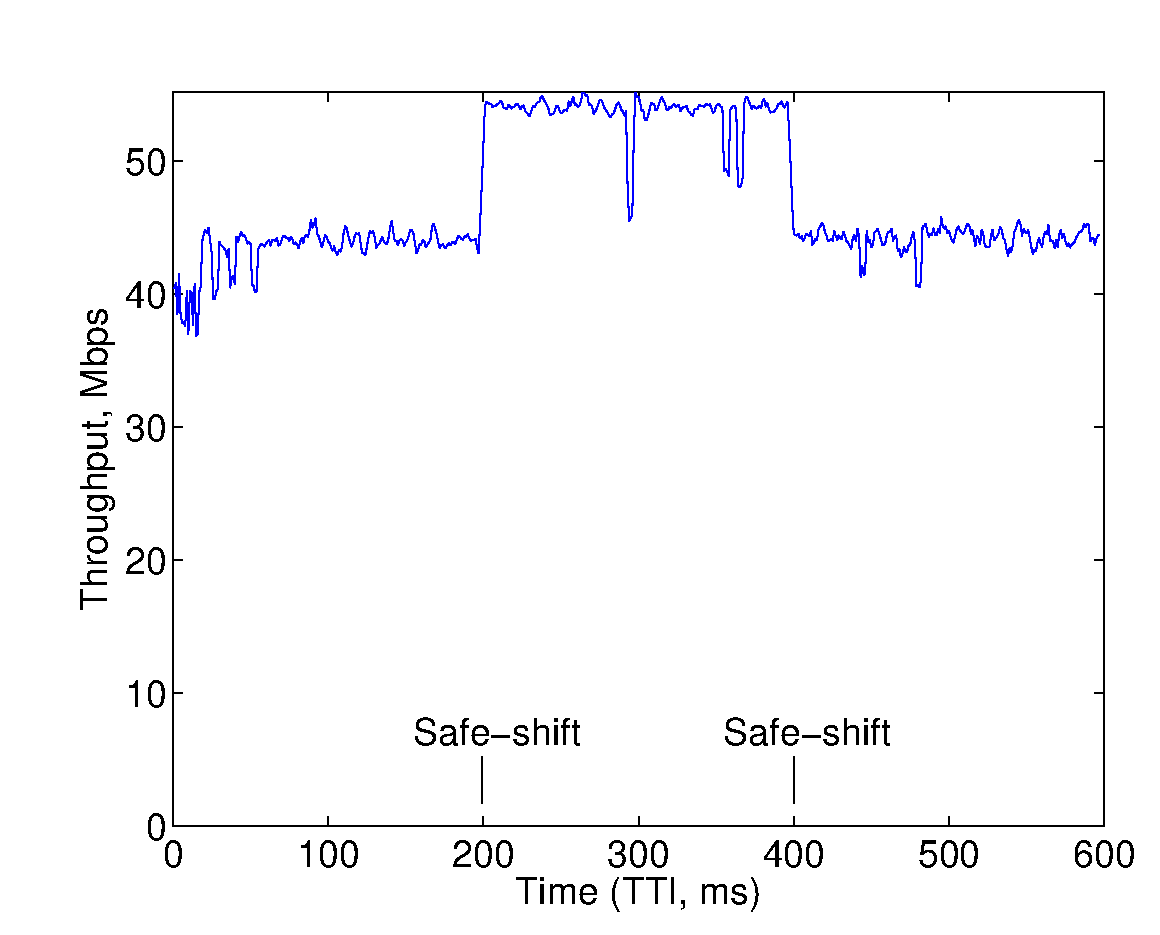
\includegraphics[width=8cm]{gcimages/overal_throughput}
    \caption{Average throughput gain. Safe-shifts are initiated at times $t_1=200$ ms and $t_2=400$ ms }
    \label{fig:safe_shift_overal_throughput}
\end{figure}

\subsection{Усиление конвергенции, ограничения перехода}
По мере обучения агентов, они постоянно изменяют свое состояние, которое в свою очередь противоречит стратегиям других агентов, делая их предположения, на которых они основаны, устаревшими. Общий подход заключается в отношении к окружающим учащимся как к части динамичной среды. Однако, это предположение ослаблено в случае параллельного обучения, где поведение других агентов, в основном, определяет саму среду.
Для преодоления господства случайного исследования над эксплуатацией, мы предлагаем следующий способ. Идея в том, чтобы предварительно заставлять агенты вести себя в уникальной манере - позволить уникальную часть состояния для каждого агента. Для этого мы предлагаем случайно проткнуть фракции $p$ $(p< 1)$ элементов матрицы перехода $TM_{ij}$ для каждого агента. Ожидается, что этот метод значительно уменьшит время сходимости процесса обучения.
Для преодоления господства случайного исследования над эксплуатацией, мы предлагаем следующий способ. Идея в том, чтобы предварительно заставлять агенты вести себя в уникальной манере - позволить уникальную часть состояния для каждого агента. Для этого мы предлагаем случайно проткнуть фракции $p$ $(p< 1)$ элементов матрицы перехода $TM_{ij}$ для каждого агента. Ожидается, что этот метод значительно уменьшит время сходимости процесса обучения.

\begin{figure}
    \centering
    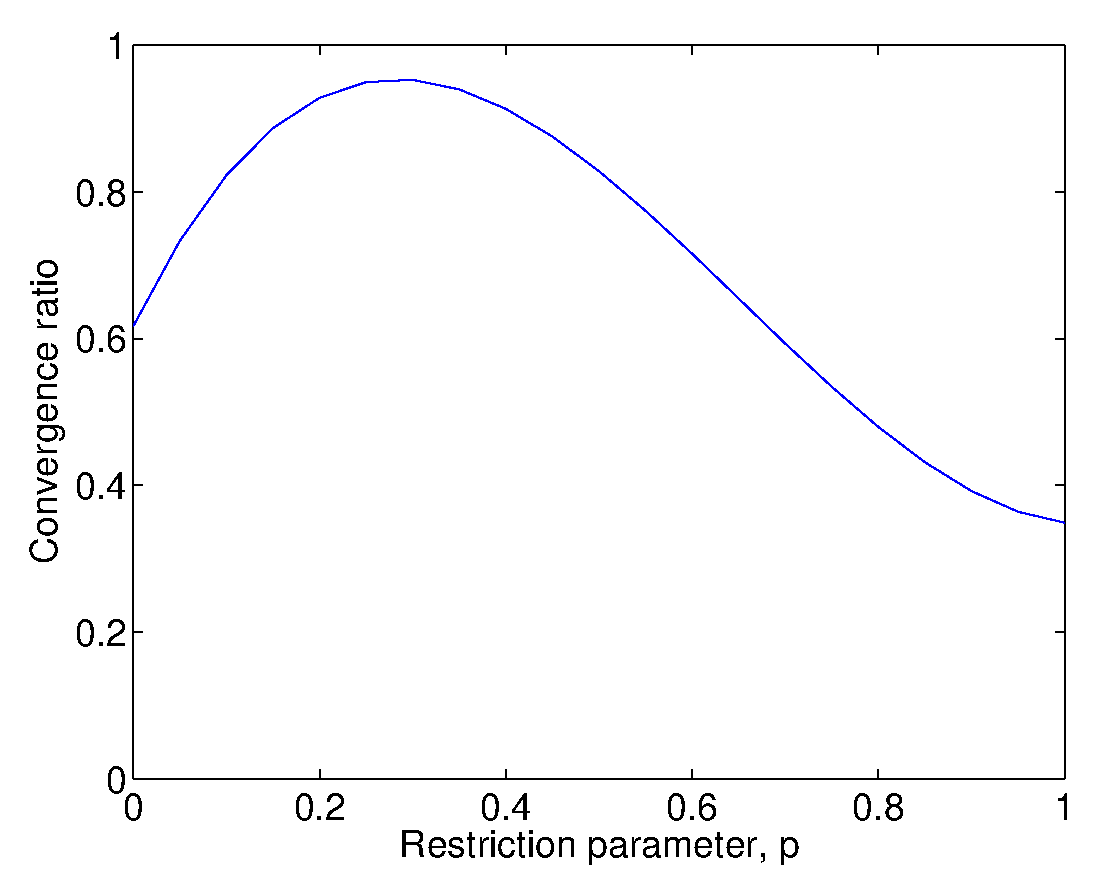
\includegraphics[width=8cm]{gcimages/restrict_p_sm}
    \caption{Average convergence ratio with puncture parameter $p$ (trend)}
    \label{fig:restrict_profit}
\end{figure}

На рисунке~\ref{fig:restrict_profit} показано соотношение сходимости усредненных за случайный набор из 500 прогонов моделирования. Под коэффициентом сходимости имеется в виду соотношение этапа эксплуатации в процессе эксплуатации системы. Значение $p = 0$ относится к случаю, когда нет ограничений к переходным правилам. Значение $p>0$ для случая, когда какая-то часть переходов случайным образом ограничена для каждого агента. Видно, что для определенного значения ($p=0.3$) коэффициент сходимости увеличивается на $20\%$.

% \subsection{Channel blocking}

\section{Оценка эффективности}

Для анализа производительности, мы проводим моделирование с помощью симулятора, основанном на Vienna LTE-A Downlink System Level Simulator (\cite{VTC2010}). Общая сеть состоит из 2-х уровневой планировки соты, где группа внутренних малых сот совмещена с базовой макро станцией. Малые соты, расположенные по сеткам 5х5, указанным в рекомендации ~\cite{R4-092042} 3GPP. Пользователи находятся в помещении и равномерно распределены. Предполагается, что каждый пользователь обслуживается базовой станцией с самым сильным сигналом. Рассмотренные каналы распространения и замирания модели основаны на ~\cite{R4-092042}. Детали моделирования по умолчанию приведены в таблице~\ref{table:simulation_parameters}.

На рисунке~\ref{fig:fcdf3} показана интегральная функция распределения пропускной способности для пользователя за количество прогонов моделирования. Предложенный алгоритм сравнивается с алгоритмом обучения, описанным в~\cite{mab}, где базовые станции принимают решения о распределении поддиапазонов с учетом занятости ресурсов каждой из окружающих сот. Видно, что предлагаемый механизм безопасного сдвига способен увеличить усредненную мощности на $8 - 10\%$ без дополнительного негативного воздействия на равнодоступность.

\begin{table}
\centering
    \caption{Simulation parameters}
    \begin{tabular}{|l l|} 
    \hline
    \textbf{Parameter} & \textbf{Description} \\
    \hline
    \multicolumn{2}{|c|}{\textbf{Scenario details}} \\
    \hline
    Base scenario & 5x5 Grid~\cite{R4-092042} \\
    \hline
    Tx power & 23 dBm \\
    \hline
    Number of eNodeBs & 7 \\
    \hline
    Number of users & 28 \\
    \hline
    Scheduler & Proportional Fair \\
    \hline
    Traffic & Best effort \\
    \hline
    Type of the antennas & Omnidirectional \\
    \hline
    RB Bandwidth & 20 Mhz \\
    \hline
    TTI duration & 1 ms \\
    \hline
    Duration of the simulation & 300 TTI, 1 h \\
    \hline
    \multicolumn{2}{|c|}{\textbf{Channel model}} \\
    \hline
    Carrier frequency & Band 7 \\
    \hline
    UE thermal noise density & -174 dBm/Hz \\
    \hline
    Shadowing fading & Log-normal, 8 dB \\
    \hline
    Fast fading & Flat fading \\
    \hline
    \multicolumn{2}{|c|}{\textbf{Algorithm parameters}} \\
    \hline
    $\alpha$ & 0.1 \\
    \hline
    $\beta$ & 0.05 \\
    \hline
    Puncture factor, $p$ & 0.3 \\
    \hline
    \end{tabular}
    \label{table:simulation_parameters}
\end{table}

Эффективность предложенного алгоритма по сравнению с традиционной статической схемой разбиения полосы частот(см., например, \cite{4907410}): 

\textbf{Повторное использование 1}: каждая базовая станция должна использовать всю доступную полосу пропускания (20 МГц, см. таблицу~\ref{table:simulation_parameters}). Затем ресурсы распределены между пользователями с помощью пропорционального справедливого планировщика.

\textbf{Повторное использование 3}: каждой базовой станции выделяется треть всего доступного диапазона. Поддиапазонное распределение настроено так, что соседние базовые станции не используют перекрывающиеся поддиапазоны.

\begin{figure}
    \centering
    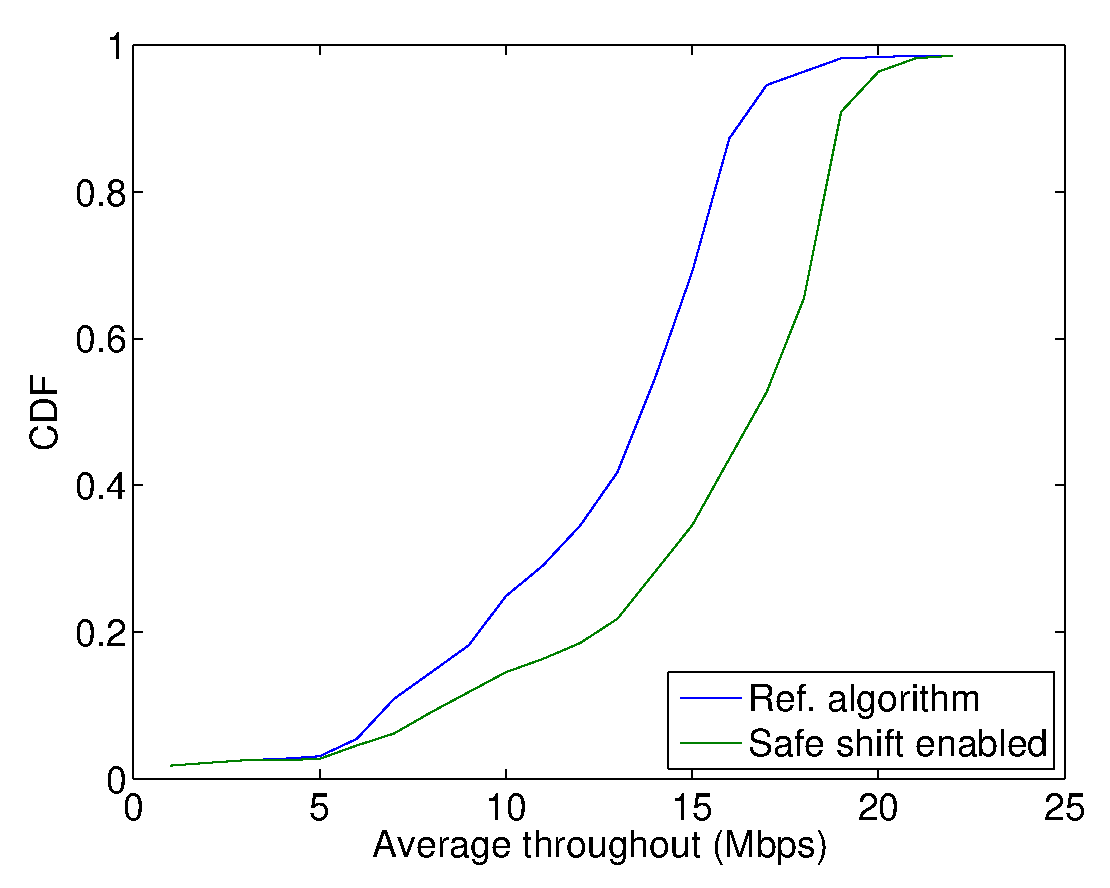
\includegraphics[width=8cm]{gcimages/fcdf3}
    \caption{CDF for average user throughput. Safe-shift gain algorithm}
    \label{fig:fcdf3}
\end{figure}

На рисунке ~\ref{fig:scdf} представлено кумулятивное распределение SINR пользователей для предлагаемого алгоритма разделения ресурсов. Значение SINR (соотношения сигнала к интерференции и шуму) рассчитывается для каждого пользователя после выделения блока ресурсов
\begin{equation}
    \label{eq:SINR}
    {SINR}_u(b) = \frac{P_u(b) G_u}{\sum_{i \in \eta} P_i(b) G_{u,i} + \sigma^2}
\end{equation}
где $P_u(b)$ - мощность передачи на поддиапазоне $b$ в соте при обслуживании пользователя $u$; $G_{u,i}$ - усиление канала между пользователем $u$ и базовой станцией $i$; и $\eta$ - это набор соседних базовых станций. Обратите внимание, что $P_i(b) = 0$, нсли базовая станция $i$ не обслуживает пользователей в поддиапазоне $b$.

\begin{figure}
    \centering
    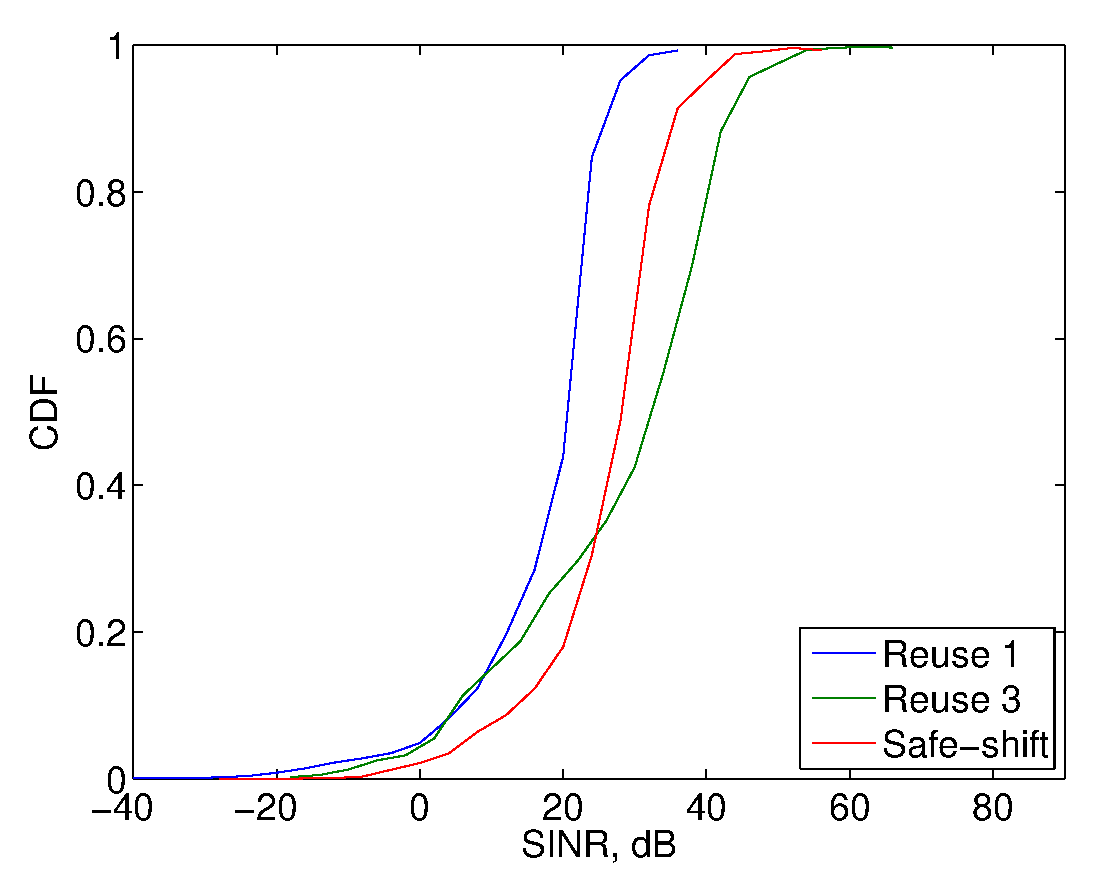
\includegraphics[width=8cm]{gcimages/scdf}
    \caption{CDF for user's SINR after resource allocation and intracell scheduling}
    \label{fig:scdf}
\end{figure}

Из рисунка~\ref{fig:scdf} можно заключить, что предложенный алгоритм способен самостоятельно найти оптимальную схему распределения поддиапазонов и превосходит традиционные централизованные статические схемы секционирования. Мы также отмечаем, что процедура безопасной смены выполняет исследование действий без вмешательства в ранее установленную схему распределения поддиапазонов. Это позволяет системе сходится к лучшему выбору без дополнительных затрат, обычно связанных с автономной разведкой. Показано, что предлагаемая процедура позволяет сократить количество случайных шагов исследования на $20\%$, несмотря на превосхождение над эталонным алгоритмом на этапе эксплуатации.

\section{Заключение}
В этой статье мы представили механизм распределения для координации интерференций между соседними сотами в плотной гетерогенной сети. Он распределяет ресурсы системы на основе мультиагентного параллельного алгоритма обучения. Основной акцент делается на сосуществование малых сотовых систем с невзаимодействующей макросредой. Мы также предложили интеллектуальное улучшение для повышения эффективности параллельных обучений за счет снижения эффекта блокировки исследования канала. Воспользовавшись так называемой процедурой безопасной смены, мы продемонстрировали способ повышения общей эффективности обучения и обеспечения сосуществования с окружающей средой в многоагентной среде.

Данный алгоритм предполагает гибкий механизм для контроля скорости сходимости в случае нескольких поддиапазонов. В качестве входных данных для алгоритма, мы используем стандарт 3GPP на основе метрик, доступных на местном уровне в каждой коммерческой малой соте, что делает его легко реализуемым на практике. Сложность алгоритма низка из-за его природы, связанной с обучением.

Моделирование на системном уровне доказало эффективность предложенного решения в условиях реалистичной установки, рекомендованных консорциумом 3GPP. В нашем исследовании мы показали, что предложенный алгоритм работает в различных разнородных сценариях и превосходит эталонные алгоритмы без негативного влияния на сходимость. Дальнейшие исследования направлены на развитие усовершенствованного алгоритма, способного динамически регулировать размеры поддиапазонов.
